\documentclass{beamer}

\usetheme{Singapore}
\usecolortheme{seahorse}

\usepackage{graphicx}
\usepackage{algpseudocode}
\usepackage{amsmath}

\graphicspath{ {./images/} }
\title{Preliminary progress on application of SLAM algorithm}
\subtitle{Offline application on Ground Vehicle}
\author{Agraj Jain  \\Hamed Ali Yaghini Bonabi}
\institute{Control/Robotics Research Laboratory}

\begin{document}

	\frame{\titlepage}
	

	\begin{frame}
		\frametitle{SLAM}
		
		\framesubtitle{Introduction}

		\begin{itemize}
			\item Localization:

			\begin{itemize}
				\item  Finding the robot's position in the environment.
			\end{itemize}

			\item Mapping:
			\begin{itemize}
				\item Creating a map of the environment.
			\end{itemize}

			\item Goal:
			\begin{itemize}
				\item  Making the robots autonomous.
				\item Creating map of the environment for different applications.
			\end{itemize}

		\end{itemize}

	\end{frame}


	\begin{frame}
		\frametitle{SLAM}
		
		\framesubtitle{Introduction}
		
		\textbf{Two general approaches:}
		\begin{itemize}
			\item Traditional approach: Metrical SLAM.
			\item  New approaches : Semantic SLAM.
		\end{itemize}

	\end{frame}


	\begin{frame}
		\frametitle{Metrical SLAM}
		
		\framesubtitle{Localization}

		\textbf{Motion Model}
		\begin{itemize}
			\item Motion model is the relation between the previous state of the robot, control inputs and the robot's current state.
		\end{itemize}
		In general:
		\begin{equation*}
			X_t=g(X_{t-1},U_t)
		\end{equation*}
where, $X_t$ is the robot's current state.$X_{t-1}$  is the robot's previous state, and $U_t$ is the control input.

	\end{frame}


	\begin{frame}
		\frametitle{Metrical SLAM}
		
		\framesubtitle{Localization}
		Simplest Localization Case: If we know the robot’s initial position \thicklines \vector(1,0){20} use the motion model for finding robot's position.! However, uncertainty in parameter’s, measurements, control.\thicklines \vector(1,0){20}  We cannot.
\textbf{General approach:}
		\begin{itemize}
			\item Motion model for Prediction.
			\item Landmarks for correction.
		\end{itemize}

	\end{frame}


	\begin{frame}
		\frametitle{Metrical SLAM}
		
		\framesubtitle{Localization}
		\textbf{Bayes Filter}
		\begin{itemize}
			\item Prediction by using motion model.
			\item Correction by landmark detection.
		\end{itemize}

		\begin{figure}
			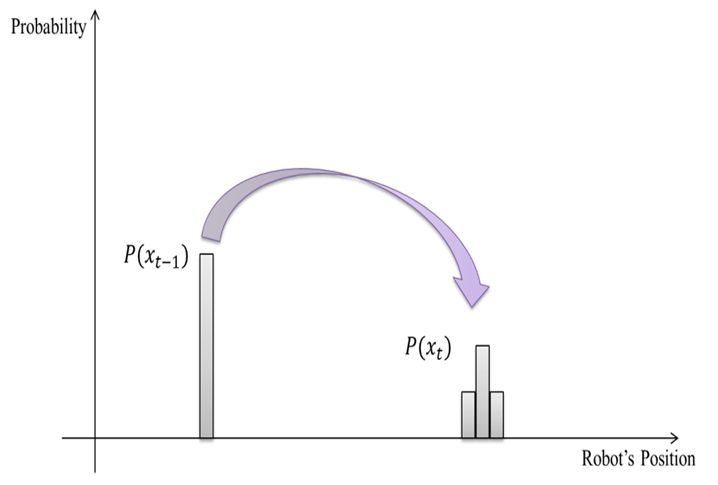
\includegraphics[width=0.6\textwidth,height=0.5\textheight]{BayesFlt}
		\end{figure}

	\end{frame}




	\begin{frame}
		\frametitle{Landmark detection}
		
		\framesubtitle{}

		\begin{itemize}
			\item Spark method: uses the step change in beam’s distance for finding landmarks.
			\item RANSAC: is used for finding walls by fitting a line to the points that are along the wall.
		\end{itemize}

	\end{frame}




	\begin{frame}
		\frametitle{Localization}
		
		\framesubtitle{Bayes Filter}

		\textbf{Bayes filter's problems:}
		\begin{itemize}
			\item Requires lots of calculation.
			\item It is discrete \thicklines \vector(1,0){20} The required memory increases by time.
		\end{itemize}
		\textbf{Solutions:}
		\begin{itemize}
			\item Selecting larger cells. \thicklines \vector(1,0){20} accuracy decreases
			\item Kalman filter.
		\end{itemize}
	\end{frame}



	\begin{frame}
		\frametitle{Localization}
		
		\framesubtitle{Kalman Filter}

		\begin{itemize}
			\item Is obtained from the Bayes filter. By assuming that robot's position has a normal distribution.
			\item Only requires calculation of mean and covariance.
		\end{itemize}

	\end{frame}




	\begin{frame}
		\frametitle{Kalman filter}
		
		\framesubtitle{Two wheeled robot}

		\textbf{Motion model}\\
		If r $\neq$ l:
		\begin{equation*}
			\alpha= \frac{r-l}{w}
		\qquad
			R=\frac{l}{\alpha}
		\end{equation*}
		\begin{equation*}
			\begin{bmatrix}
				x'\\y'\\\theta'
			\end{bmatrix}
			=
			\begin{bmatrix}
				x\\y\\\theta
			\end{bmatrix}
			+
			\begin{bmatrix}
				\left(R+\frac{w}{2}\right)(\sin(\theta+\alpha)-\sin(\theta))\\
				\left(R+\frac{w}{2}\right)(-\cos(\theta+\alpha)-\cos(\theta))\\
				\alpha
			\end{bmatrix}
		\end{equation*}	
		If r = l:
		\begin{equation*}
			\begin{bmatrix}
				x'\\y'\\\theta'
			\end{bmatrix}
			=
			\begin{bmatrix}
				x\\y\\\theta
			\end{bmatrix}
			+
			\begin{bmatrix}
				l.\cos(\theta)\\
				l.\sin(\theta)\\
				0
			\end{bmatrix}
		\end{equation*}	
		In general:
		$ x'=g(x,u) $ Where:
		\begin{equation*}
			x=
			\begin{bmatrix}
				x\\y\\\theta
			\end{bmatrix}
			\qquad
			u=
			\begin{bmatrix}
				l\\r
			\end{bmatrix}
		\end{equation*}

	\end{frame}



	\begin{frame}
		\frametitle{Extended Kalman Filter}
		\framesubtitle{Correction}
		\textbf{Predicting the measurement:}
		\begin{equation*}
			\bar{z_{t}}=h(x_m,y_m,\theta)
		\end{equation*}
		\begin{equation*}
			\bar{z}_t=\begin{bmatrix}
				r\\\alpha
			\end{bmatrix}
			=
			\begin{bmatrix}
				\sqrt{(x_l-x_m)^2+(y_l-y_m)^2}\\
				\arctan\left(\frac{y_l-y_m}{x_l-x_m}\right)-\theta
			\end{bmatrix}
		\end{equation*}
		Where, $ x_m,y_m $ are the co-ordinates of each landmark already on the map. 
	\end{frame}





	\begin{frame}
		\frametitle{Extended Kalman filter}
		
		\framesubtitle{}
		EKF's problems:
		\begin{itemize}
			\item What will happen if we don’t know the robot's initial position ? What if the position’s distribution is not normal?
		\end{itemize}
		\thicklines \vector(1,0){20}Particle filter
The main idea: using points and their density as a tool for representing distribution
	\end{frame}



	\begin{frame}
		\frametitle{Simultaneous localization and mapping}
		
		\framesubtitle{}

		\begin{itemize}
			\item Put the world coordinates’ origin in the robot's starting point.
			\item Start observing the environment.
			\item While moving, add the landmarks as detected to the system’s state, with uncertainty.
			\item Use prediction and correction methods of localization to finding the correct location of both robot and landmarks.
		\end{itemize}
		\begin{equation*}
			\mu=
			\begin{bmatrix}
				x\\y\\\theta\\x_1\\y_1\\x_2\\y_2\\.\\.\\.
			\end{bmatrix}
		\end{equation*}

	\end{frame}













	\begin{frame}
		\frametitle{Implementation}
		
		\framesubtitle{Ground Vehicle basics}
		
		\begin{figure}
			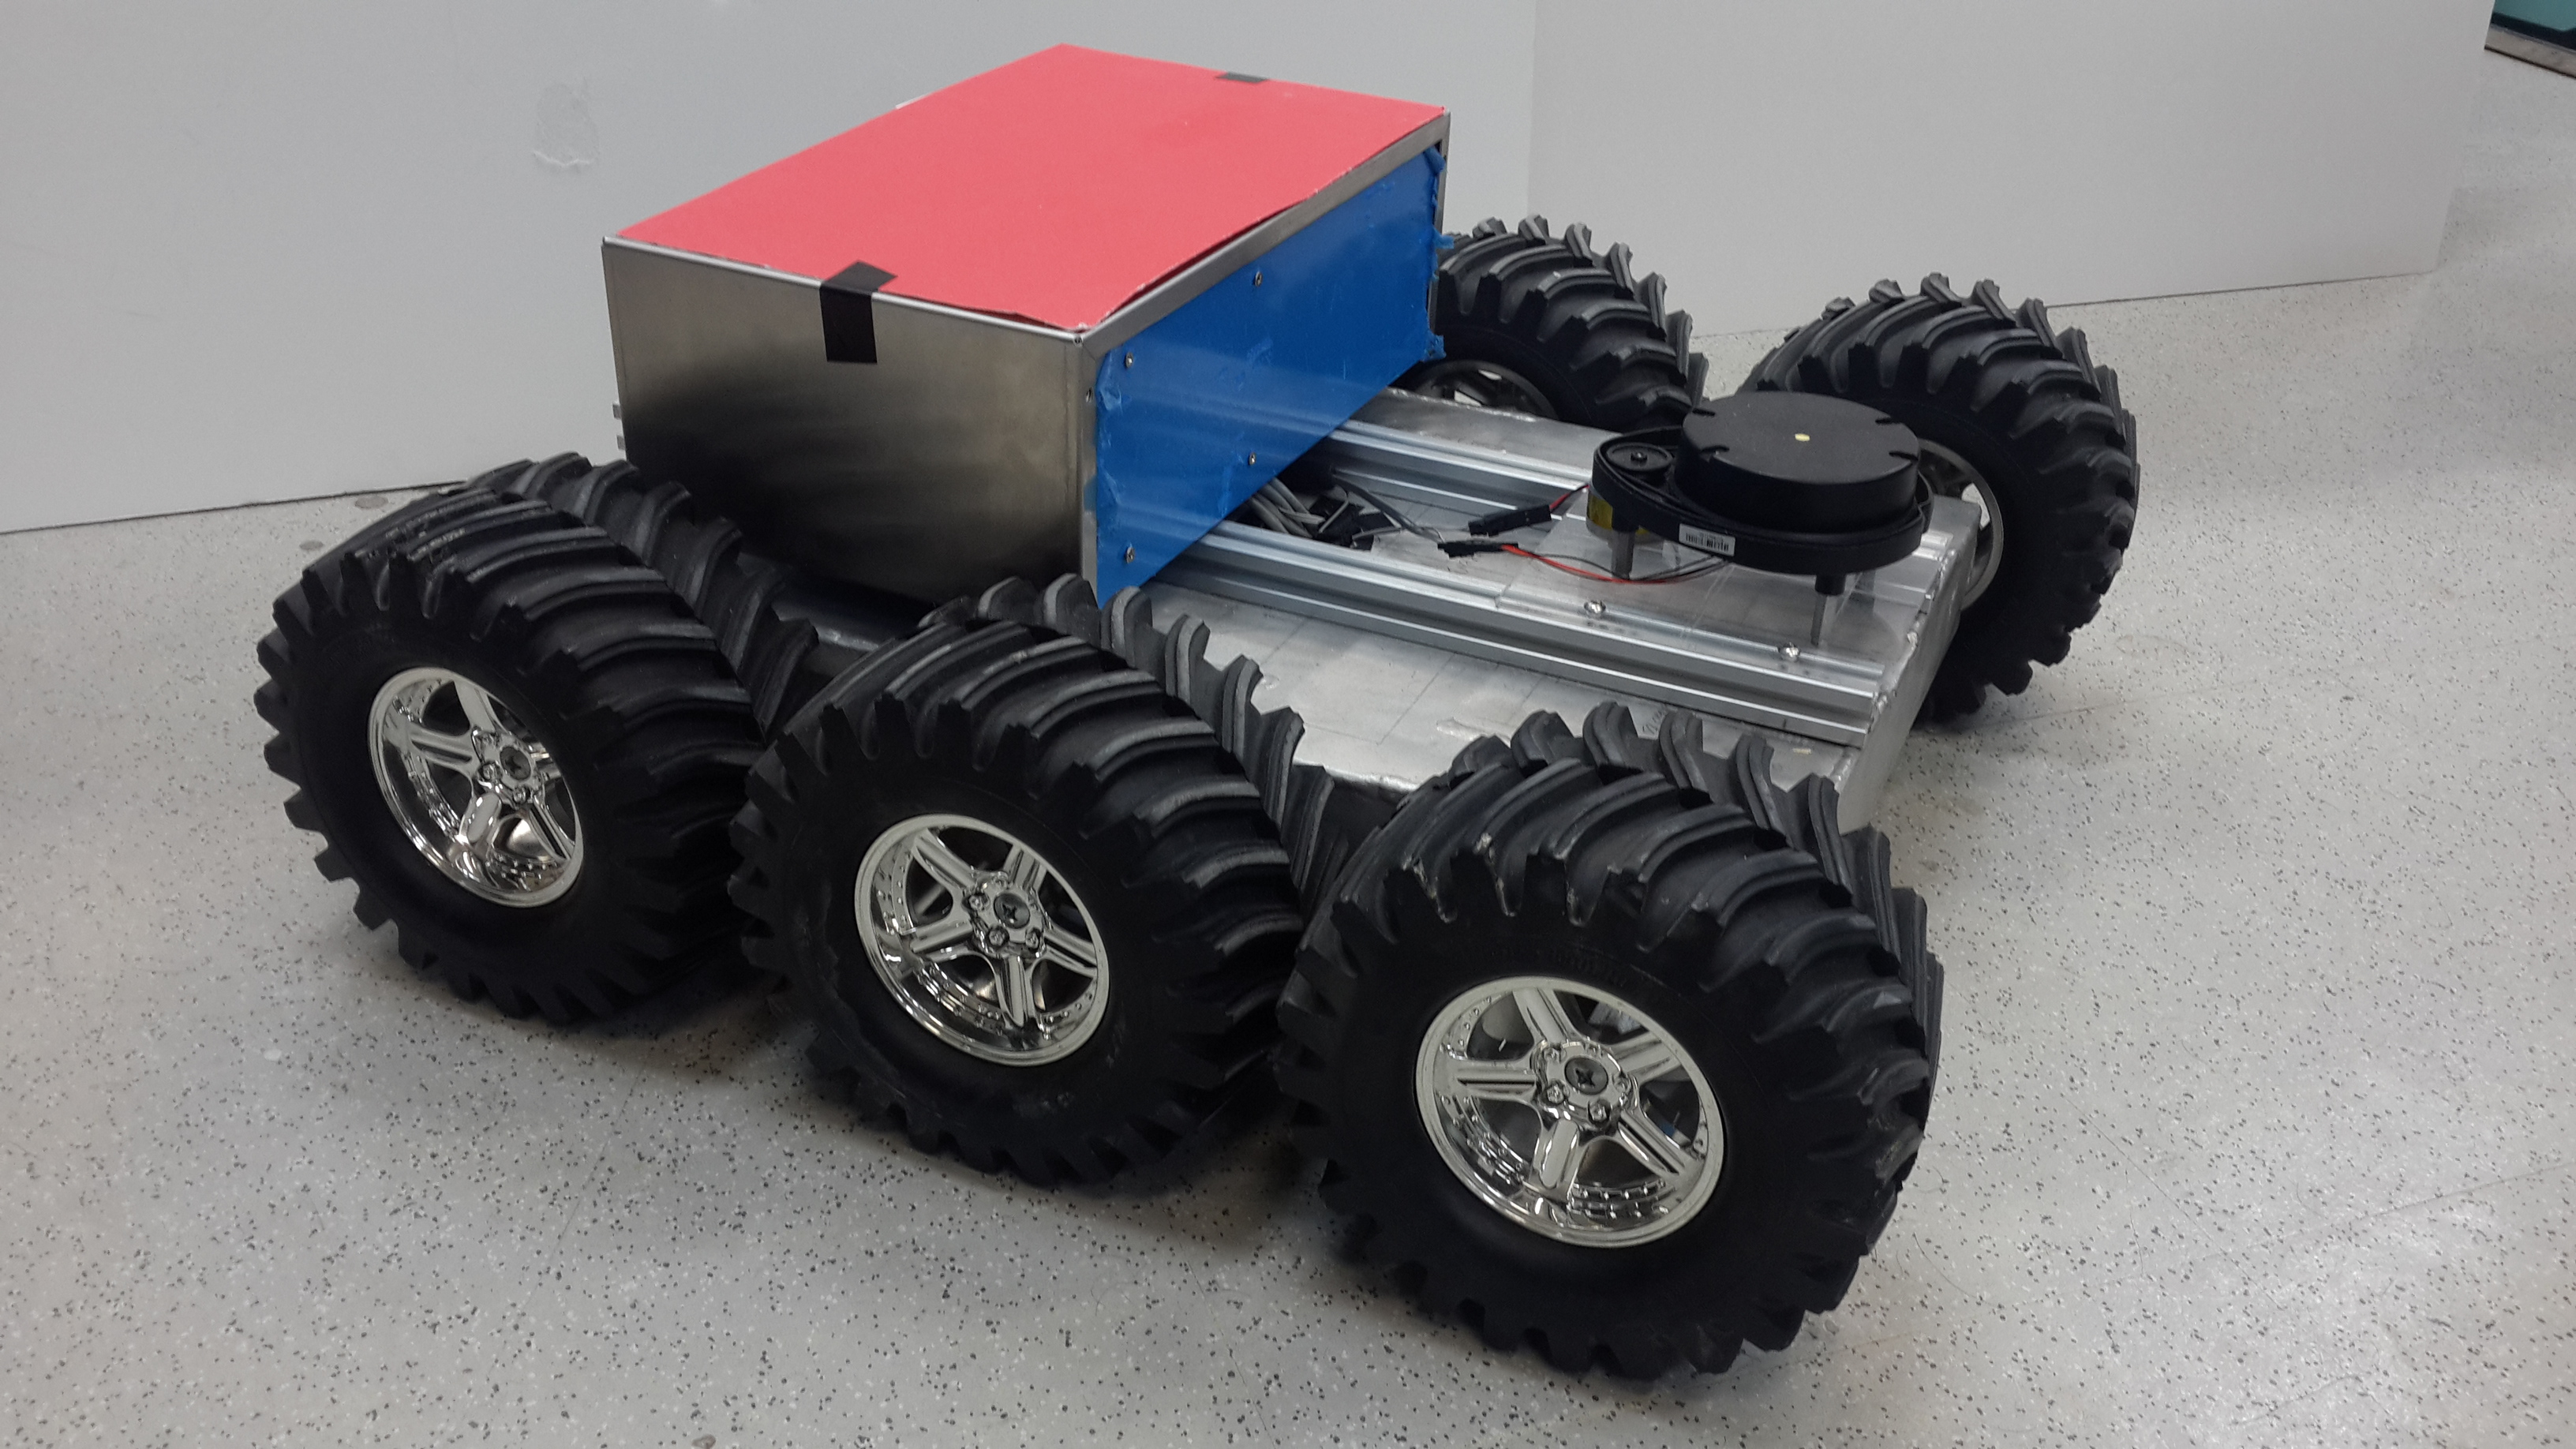
\includegraphics[width=0.4\textwidth,height=0.4\textheight]{GMM}
		\end{figure}

		\begin{itemize}
			\item Odometry:
				\begin{itemize}
					\item 2 Encoders sampled at 1000 Hz
					\item Velocity logged at a rate of 200 Hz
				\end{itemize}
			\item Piccolo Laser Distance Sensor:
				\begin{itemize}
					\item 6 m range
					\item 5 Hz Rotation Speed
					\item 1$\deg$ Angular Resolution
				\end{itemize}
		\end{itemize}
	\end{frame}
	
	\begin{frame}
		\frametitle{Implementation}
		
		\framesubtitle{Enviornment}
		
		\begin{figure}
			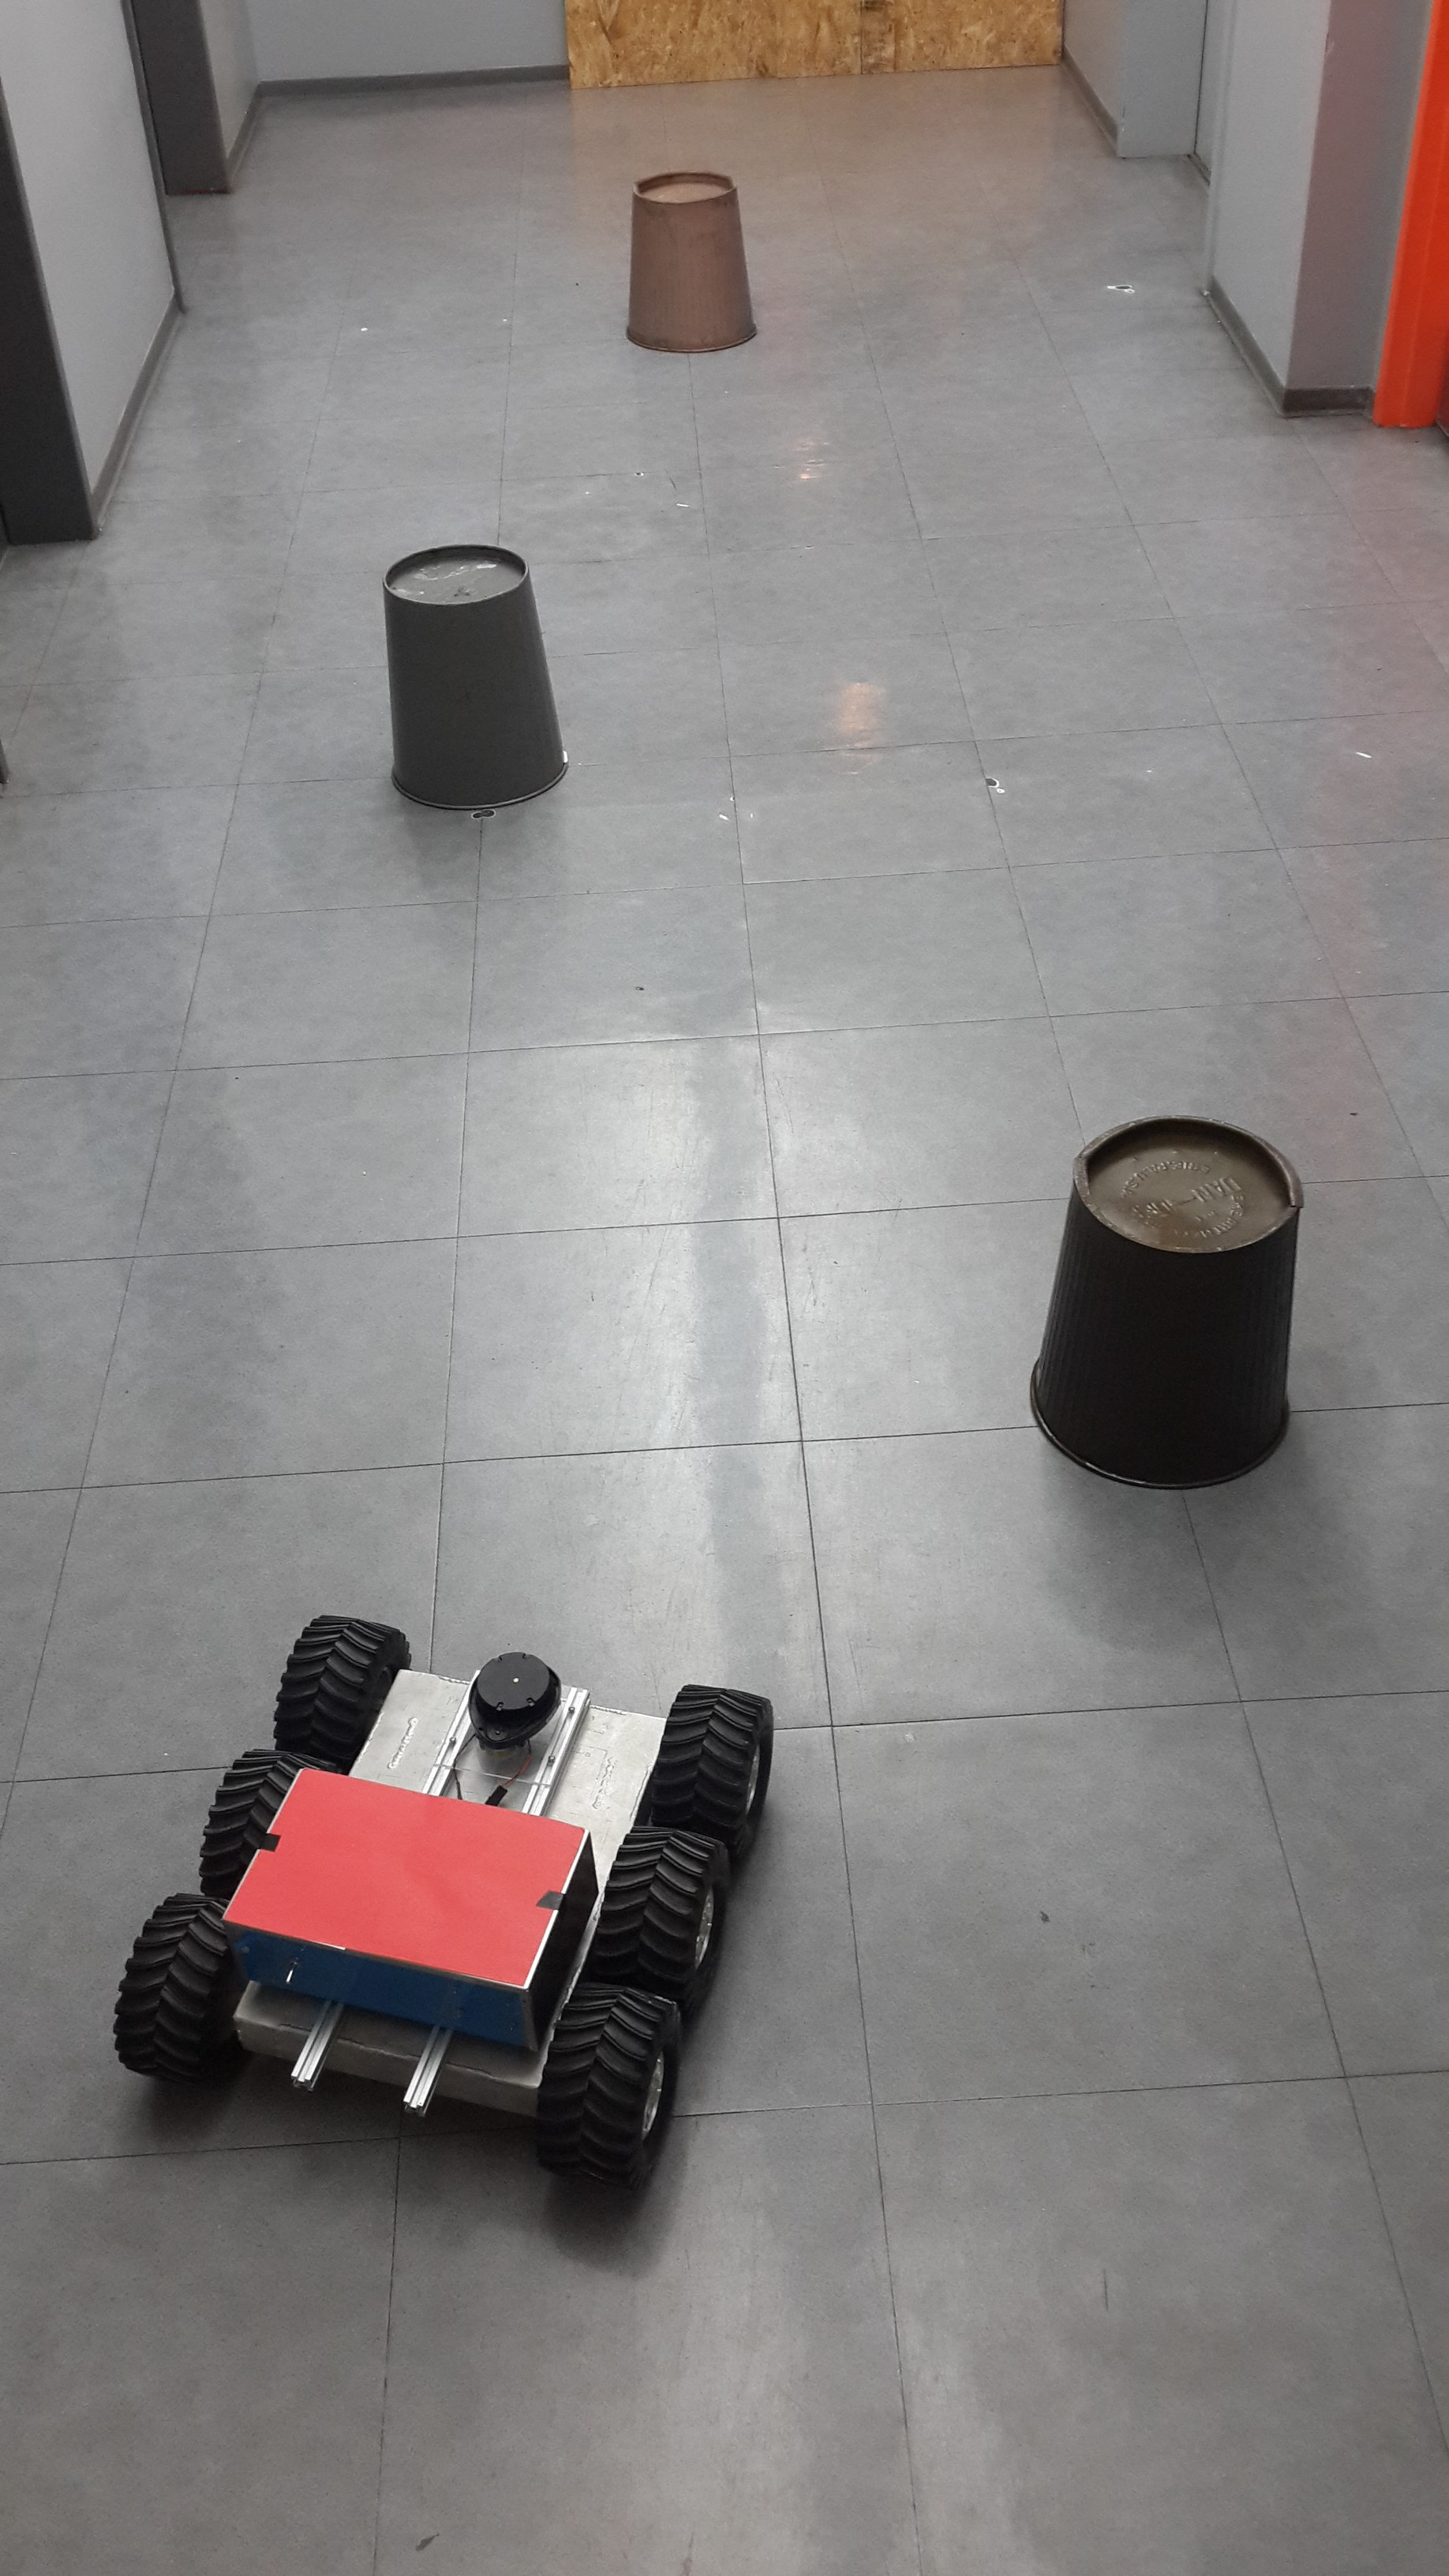
\includegraphics[width=0.4\textwidth,height=0.7\textheight]{Full}
		\end{figure}
		
	\end{frame}

	\begin{frame}
		\frametitle{Landmark Extraction methods}
		\framesubtitle{Spike Landmark Extraction}
		\begin{figure}
			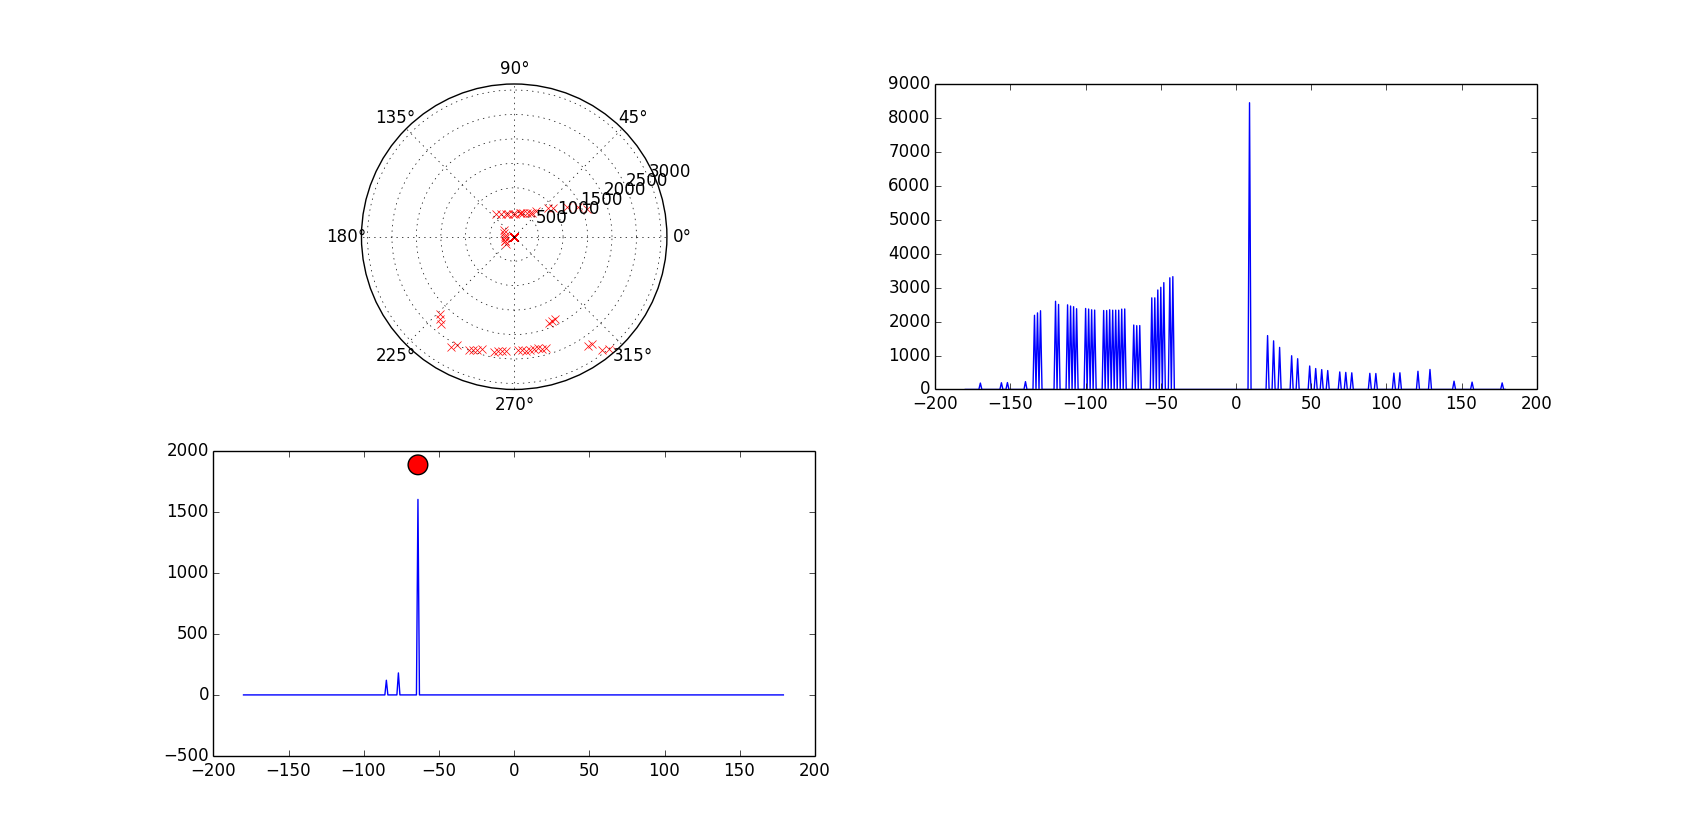
\includegraphics[width=0.6\textwidth,height=0.4\textheight]{spike}
		\end{figure}
		\begin{itemize}
			\item Derivative Based Detection
			\item Very susceptible to noise
			\item Dependent on environment and shape of landmark
		\end{itemize}
	\end{frame}

	\begin{frame}
		\frametitle{Landmark Extraction methods}
		\framesubtitle{RANSAC}
		\textbf{Traditional Algorithm:}\footnote{From wikipedia}
		\begin{enumerate}
		\item Select a random subset of the original data. Call this subset the hypothetical inliers.
		\item A model is fitted to the set of hypothetical inliers.
		\item All other data are then tested against the fitted model. Those points that fit the estimated model well, according to some model-specific loss function, are considered as part of the consensus set.
		\item The estimated model is reasonably good if sufficiently many points have been classified as part of the consensus set.
		\item Afterwards, the model may be improved by reestimating it using all members of the consensus set.
		\end{enumerate}
	\end{frame}
	
		\begin{frame}[shrink]
			\frametitle{Landmark Extraction methods}
			\framesubtitle{RANSAC}
			\textbf{Algorithm used:}
			\begin{algorithmic}
				\While{
				\begin{itemize}
					\item there are still unassociated laser readings, 
					\item and the number of readings is larger than the consensus, 
					\item and we have done less than N trials.
				\end{itemize}
				}
				\begin{itemize}
				\item Select a random laser data reading. 
				\item Randomly sample S data readings within D degrees of this laser 
				data reading 
				\item Using these S samples and the original reading calculate a 
				least squares best fit line. 
				\item Determine how many laser data readings lie within X distance 
				from this best fit line
				\item If the number of laser data readings on the line is above some 
				consensus C do the following: 
					\begin{itemize}
						\item calculate new least squares best fit line based on all 
						the laser readings determined to lie on the old best fit 
						line. 
						\item Add this best fit line to the lines we have extracted. 
						\item Remove the number of readings lying on the line from the 
						total set of unassociated readings.
					\end{itemize}
				\end{itemize}
				\EndWhile
			\end{algorithmic}
		\end{frame}
		
		\begin{frame}
			\frametitle{Landmark Extraction methods}
			\framesubtitle{RANSAC}
			\begin{figure}
				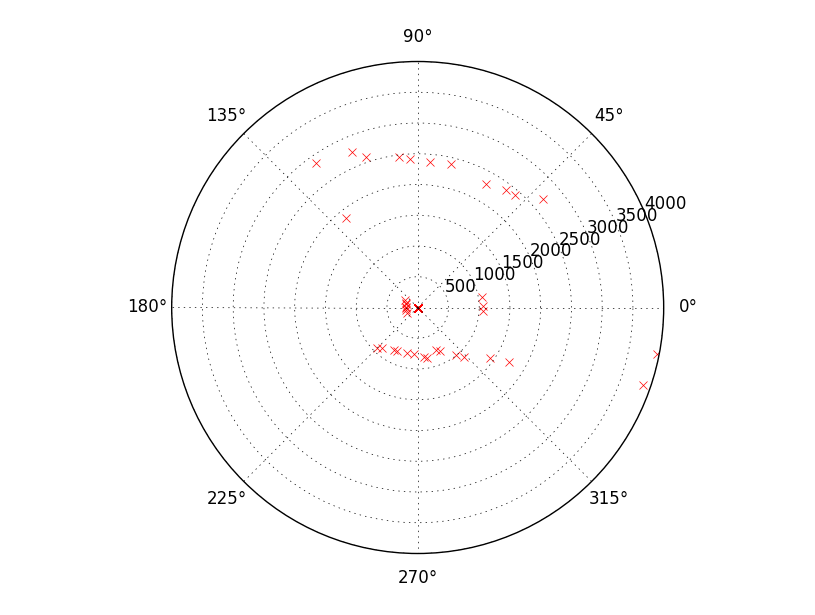
\includegraphics[width=0.7\textwidth,height=0.7\textheight]{1Scan}
				\caption{The LIDAR Scan}
			\end{figure}
		\end{frame}
		
		\begin{frame}
			\frametitle{Landmark Extraction methods}
			\framesubtitle{RANSAC}
			\begin{figure}
				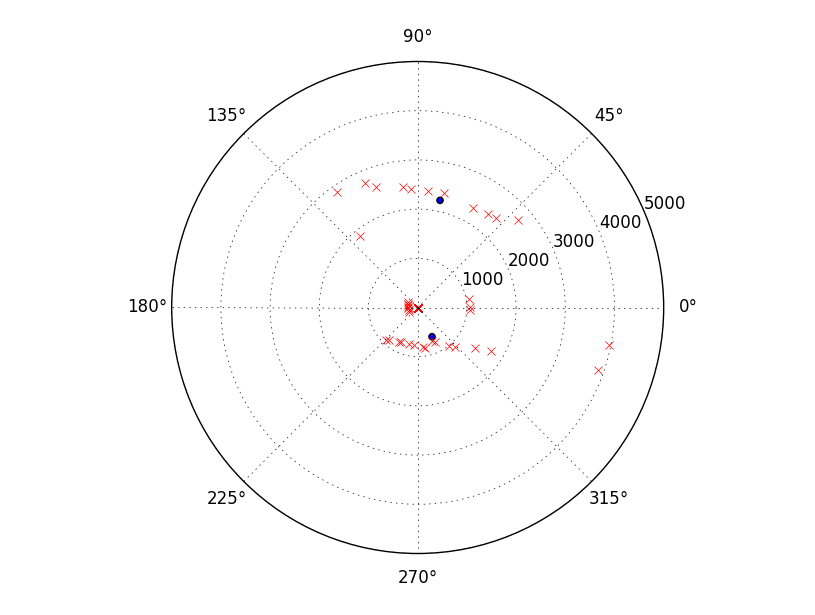
\includegraphics[width=0.7\textwidth,height=0.7\textheight]{2Walls}
				\caption{Detected walls}
			\end{figure}
		\end{frame}
		
		\begin{frame}
			\frametitle{Landmark Extraction methods}
			\begin{figure}
				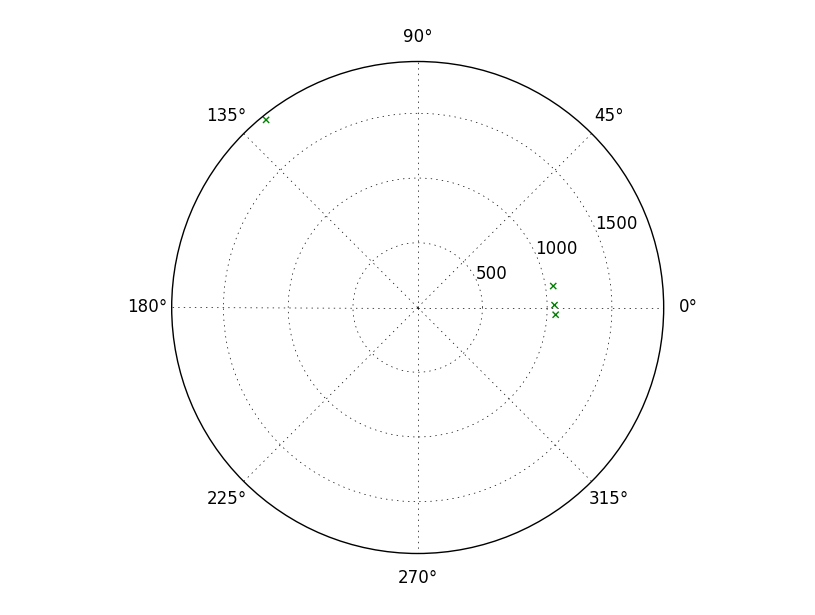
\includegraphics[width=0.7\textwidth,height=0.7\textheight]{3Unass}
				\caption{Remaining points}
			\end{figure}
		\end{frame}
				
		\begin{frame}
			\frametitle{Landmark Extraction methods}
			\framesubtitle{Mean Shift Clustering}
			\begin{itemize}
				\item Centroid based algorithm
				\item  Works by updating candidates for centroids to be the mean of the points within a given region
			\end{itemize}
			Given a candidate centroid $x_i$ for iteration $t$, the candidate is updated according to the following equation:
			\begin{equation*}
				x_i^{t+1}=x_i^t+m(x_i^t)
			\end{equation*}
			m is the mean shift vector that is computed for each centroid that points towards a region of the maximum increase in the density of points.
			\begin{equation*}
				m(x_i)=\frac{\sum_{x_j \in N(x_i)}K(x_j-x_i)x_j}{\sum_{x_j \in N(x_i)}K(x_j-x_i)}
			\end{equation*}
		\end{frame}
		
		\begin{frame}
			\frametitle{Landmark Extraction methods}
			\begin{figure}
				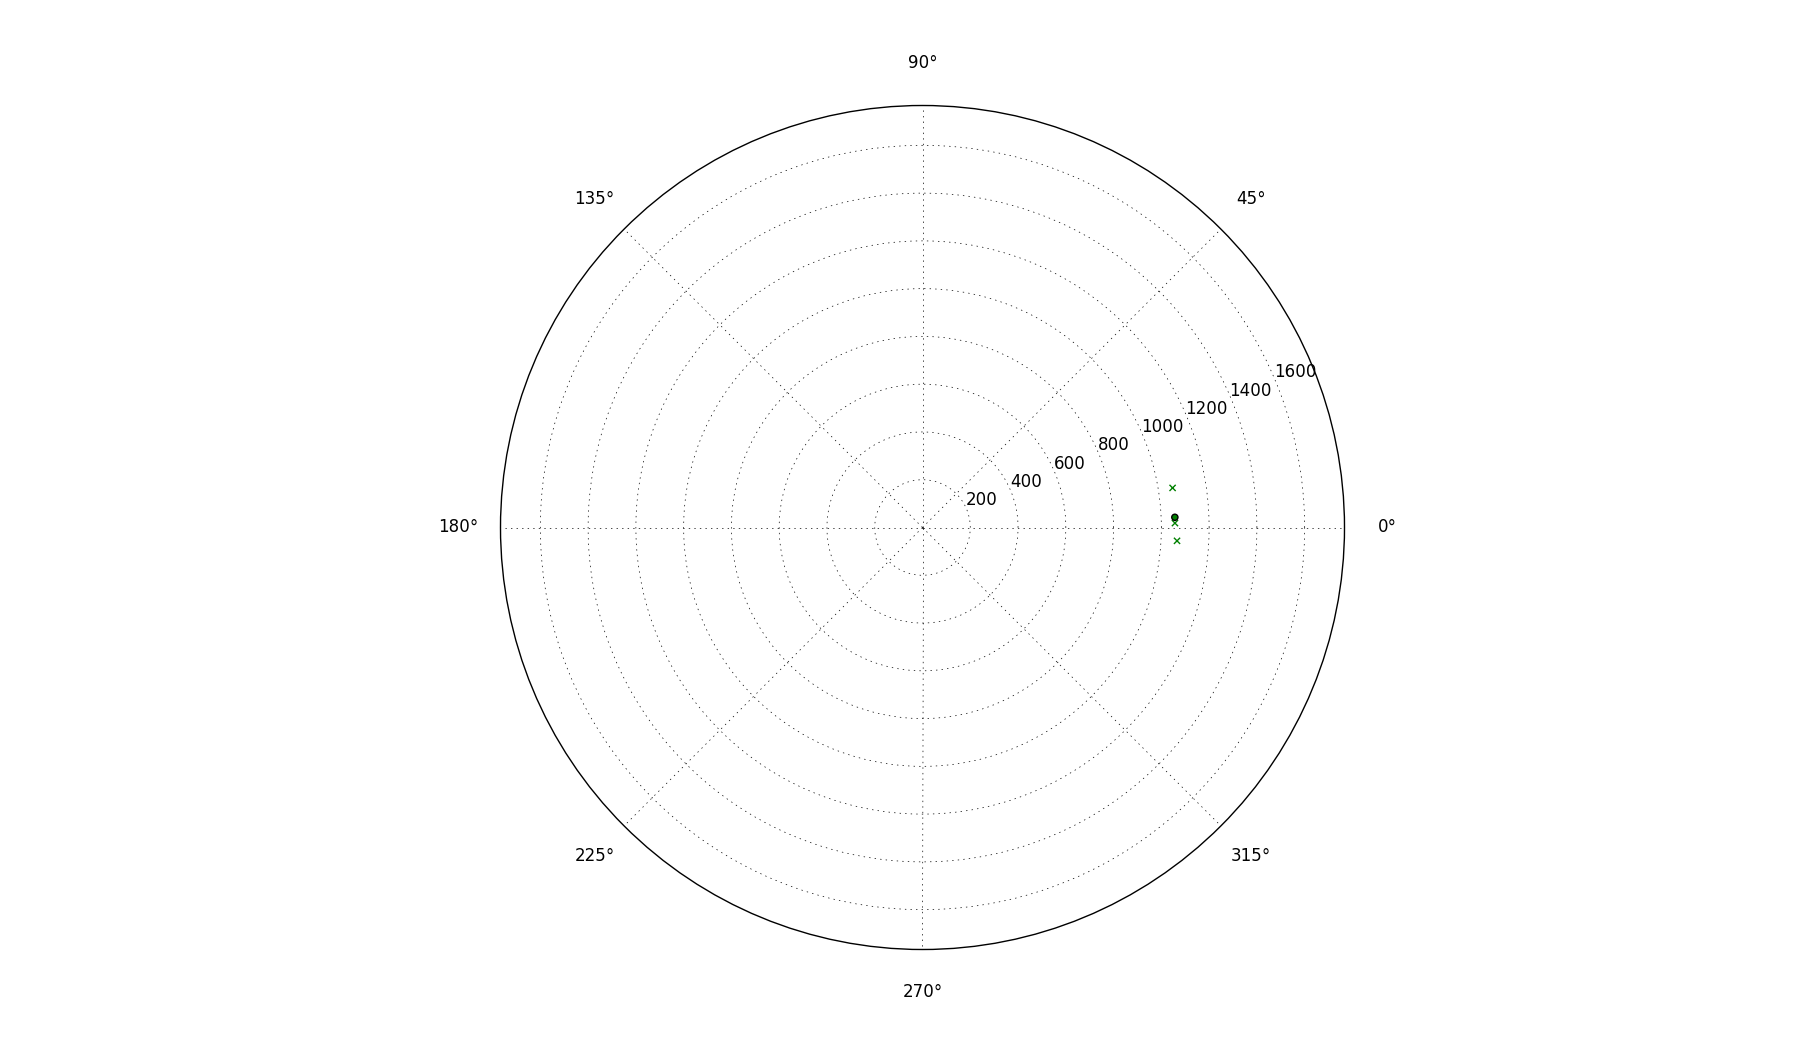
\includegraphics[width=0.7\textwidth,height=0.7\textheight]{4Cyl}
				\caption{Detected Cylinders}
			\end{figure}
		\end{frame}
		
		\begin{frame}
			\frametitle{Results}
			\begin{figure}
				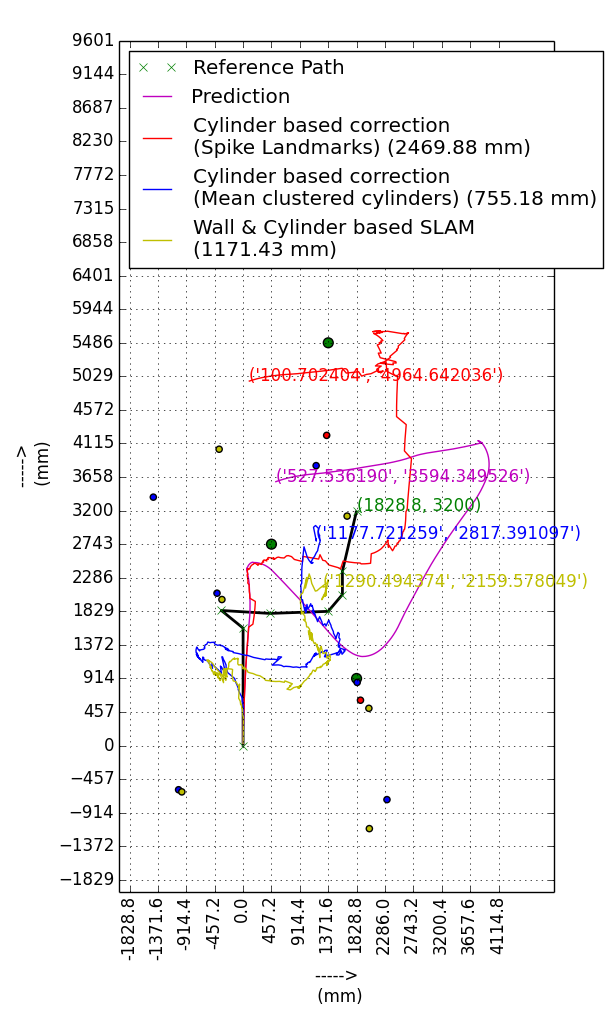
\includegraphics[width=0.4\textwidth,height=0.7\textheight]{overlayResult}
			\end{figure}
		\end{frame}
		
		\begin{frame}
			\frametitle{Future Landmark Extraction methods}
			\framesubtitle{Feature detection}
			\begin{figure}
				\centering
				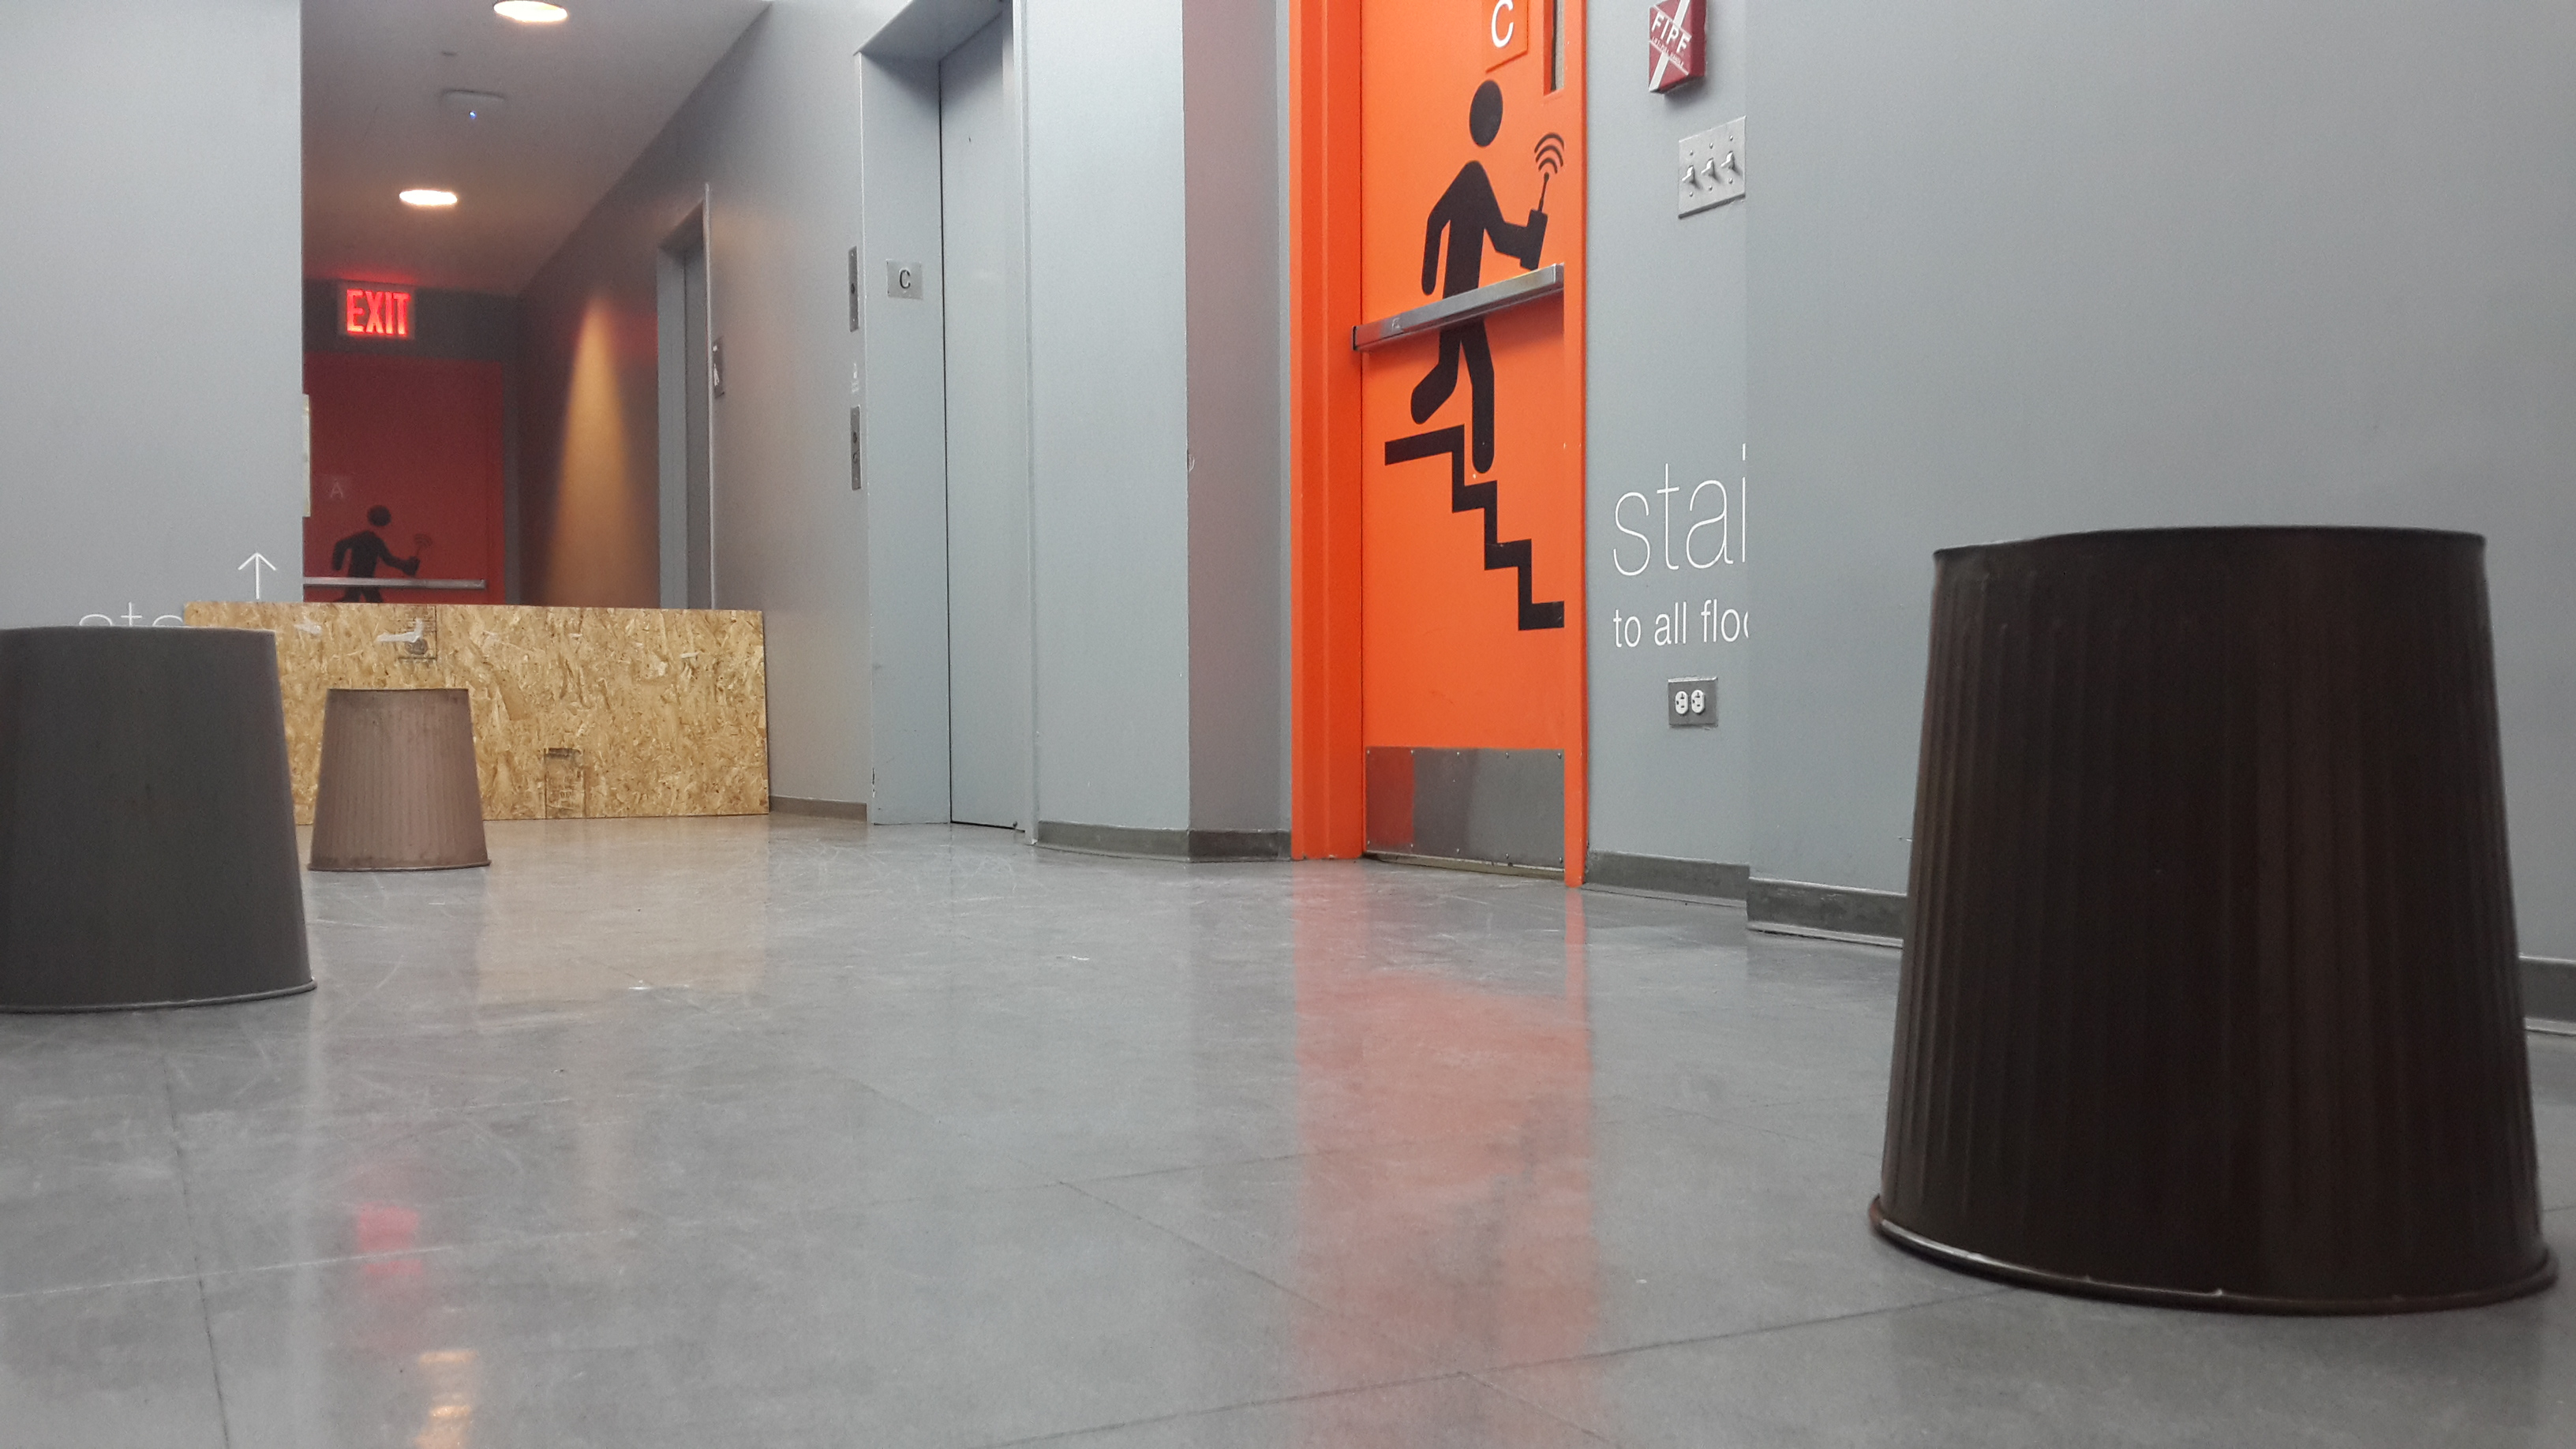
\includegraphics[width=0.7\textwidth,height=0.7\textheight]{onboard}
				\caption{Typical on-board camera frame}
			\end{figure}

		\end{frame}





	\begin{frame}
		\frametitle{Semantic SLAM}
		
		\framesubtitle{}
		\textbf{Difference with metrical SLAM}
		\begin{itemize}
			\item Metrical SLAM: looks at geographical position of the landmarks == sees them as obstacle, does not interpret sensor information other than the geometric level.
			\item Semantic SLAM: uses other features of environment for producing a meaningful representation.
		\end{itemize}

	\end{frame}






	\begin{frame}
		\frametitle{Semantic SLAM}
		
		\framesubtitle{}

		 Applications:
			\begin{itemize}
				\item Possibility of information sharing between robots, and robots and humans  \thicklines \vector(1,0){20}
				\begin{itemize}
					\item Human robot collaboration.
					\item Collaboration of robots with each other.
				\end{itemize} 
			\end{itemize}

		The richer the environment model, and the higher its semantic level \thicklines \vector(1,0){20} the more useful it becomes for a robot in order to perform autonomous tasks.


	\end{frame}





	\begin{frame}
		\frametitle{Semantic SLAM}
		
		\framesubtitle{Examples}
		Meaningful representation \thicklines \vector(1,0){20} distinguishing navigable and non navigable areas.
		\begin{figure}
			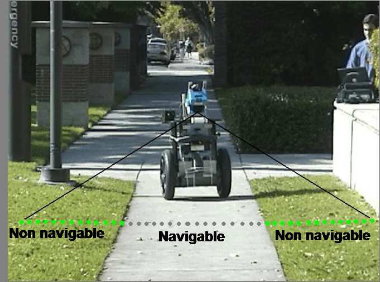
\includegraphics[width=0.5\textwidth,height=0.6\textheight]{Navigable}
		\end{figure}
	\end{frame}




	\begin{frame}
		\frametitle{Semantic SLAM}
		
		\framesubtitle{Applications}
Collaboration between robots.
		\begin{itemize}
			\item Aerial Robots
			\item Ground Robots
		\end{itemize}

	\end{frame}





	\begin{frame}
		\frametitle{Thank you}
	\end{frame}	



\end{document}